\documentclass[12pt, a4paper, oneside]{book} % 定义文档类和选项
\usepackage[UTF8]{ctex} % 引入支持中文的宏包

\usepackage[headheight=15pt,   % 页眉高度（根据实际页眉内容调整）
    footskip=30pt,     % 页脚基线到版心底部的距离
    top=2.5cm,         % 上边距（包含页眉）
    bottom=2.5cm,      % 下边距（包含页脚）
    left=2.5cm,        % 左边距
    right=2.5cm,
    includeheadfoot]{geometry}

\usepackage{fancyhdr}  % 导入 fancyhdr 宏包

% 设置页眉和页脚
\pagestyle{fancy}
\fancyhf{}  % 清除所有默认页眉页脚内容

\fancyhead[L]{Q群~1029757969}

\fancyfoot[R]{B站ID 礼貌小猫咪}


\renewcommand{\headrulewidth}{0pt} 


\usepackage[hidelinks]{hyperref}
\usepackage{bookmark}

\usepackage{tkz-euclide} %为几何画图设计的宏包
\usetikzlibrary{calc} % 坐标计算功能
\usetikzlibrary{intersections} % 交点计算功能
\usetikzlibrary{arrows.meta} %箭头
\tikzset{>={Stealth[scale=1.4]}} %燕尾箭头
\usepackage[most]{tcolorbox}
\usepackage[svgnames]{xcolor}

\usepackage{titlesec} 
\titleformat{\chapter}[display]
{\normalfont\LARGE\bfseries\raggedright}{\chaptertitlename\ \thechapter}{10pt}{\Large}

\titleformat{\section}
{\normalfont\large\bfseries}{\thesection}{1em}{}

\titleformat{\subsection}
{\normalfont\bfseries}{\thesubsection}{1em}{}


\title{\LaTeX{} GeoTikTrim \thanks{项目地址: \url{https://gitee.com/Jack0920/ggb-tikz-code-filter}}} % 
\author{Jack}
\date{\today}
\begin{document} 
\maketitle

\tableofcontents

\newpage
\chapter{version 0.0.4}
\newpage
\section{函数以及文本标签}
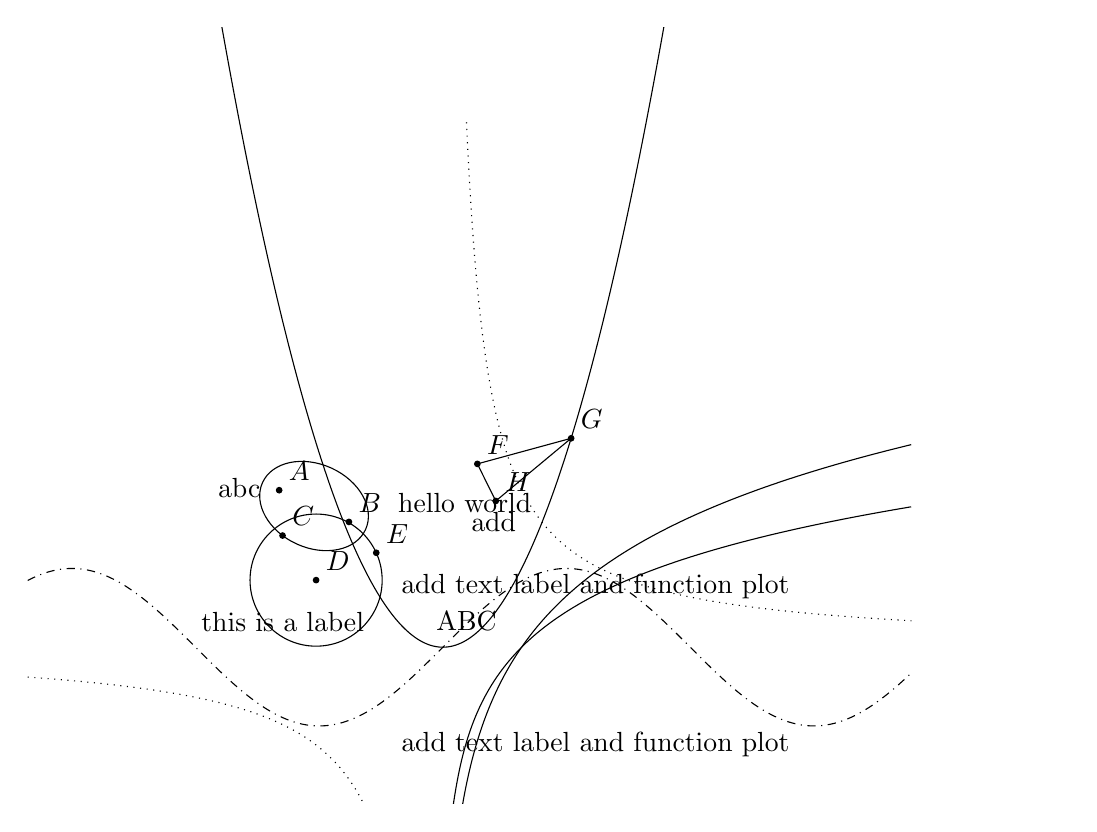
\begin{tikzpicture}[scale=1]
  % 坐标点定义
  \coordinate (A) at (-2.079,1.994);
  \coordinate (B) at (-1.193,1.591);
  \coordinate (C) at (-2.036,1.418);
  \coordinate (D) at (-1.61,0.852);
  \coordinate (E) at (-0.846,1.199);
  \coordinate (F) at (0.438,2.328);
  \coordinate (G) at (1.629,2.653);
  \coordinate (H) at (0.672,1.857);

  % 函数图像
  \begin{scope}
    \clip(-5.273,-1.988) rectangle (7.951,7.868);
    \draw[dash dot,smooth,samples=500,domain=-5.273:5.951] plot(\x,{sin(((\x))*180/pi)});
    \draw[dotted,smooth,samples=500,domain=-5.273:-0.3] plot(\x,{2/(\x)});
    \draw[dotted,smooth,samples=500,domain=0.3:5.951] plot(\x,{2/(\x)});
    \draw[smooth,samples=500,domain=0.001:5.951] plot(\x,{ln((\x))});
    \draw[smooth,samples=500,domain=0.001:5.951] plot(\x,{ln((\x))/ln(2)});
    \draw[smooth,samples=500,rotate around={0:(0,0)},domain=-4:4] plot(\x,{(\x)^2/2/0.5});
  \end{scope}

  % 几何元素
  \draw (D) circle (0.839cm);

  % 椭圆
  \draw[rotate around={-24.471:((-1.636,1.793))}] (-1.636,1.793) ellipse (0.719cm and 0.53cm);

  \draw (F) -- (G);
  \draw (G) -- (H);
  \draw (H) -- (F);

  % 点标记
  \draw[fill=black] (A) circle (1pt);
  \draw[fill=black] (B) circle (1pt);
  \draw[fill=black] (C) circle (1pt);
  \draw[fill=black] (D) circle (1pt);
  \draw[fill=black] (E) circle (1pt);
  \draw[fill=black] (F) circle (1pt);
  \draw[fill=black] (G) circle (1pt);
  \draw[fill=black] (H) circle (1pt);

  % 点标签
  \node [above right] at (A) {$A$};
  \node [above right] at (B) {$B$};
  \node [above right] at (C) {$C$};
  \node [above right] at (D) {$D$};
  \node [above right] at (E) {$E$};
  \node [above right] at (F) {$F$};
  \node [above right] at (G) {$G$};
  \node [above right] at (H) {$H$};

  % 文本标签
  \draw (-0.652,1.046) node[anchor=north west] {add text label and function plot};
  \draw (-0.652,1.046) node[anchor=north west,shift={(0,-2)}] {add text label and function plot};
  \draw (0.238,1.835) node[anchor=north west] {add};
  \draw (-0.692,2.077) node[anchor=north west] {hello world};
  \draw (-3.19,0.571) node[anchor=north west] {this is a label};
  \draw (-2.978,2.27) node[anchor=north west] {abc};
  \draw (-0.207,0.571) node[anchor=north west] {ABC};
\end{tikzpicture}

\chapter{version 0.0.5}
\begin{enumerate}
  \item 优化了点标签的位置
  \item 新增绘制扇形
\end{enumerate}

\newpage

\section{优化点标签位置}
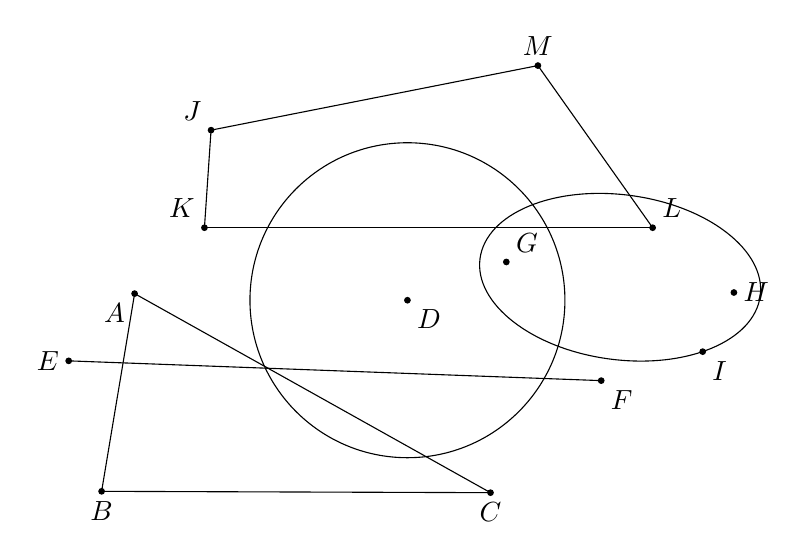
\begin{tikzpicture}[scale=1]
  % 坐标点定义
  \coordinate (A) at (-1.611,2.986);
  \coordinate (B) at (-2.03,0.475);
  \coordinate (C) at (2.909,0.458);
  \coordinate (D) at (1.854,2.902);
  \coordinate (E) at (-2.448,2.132);
  \coordinate (F) at (4.315,1.881);
  \coordinate (G) at (3.11,3.388);
  \coordinate (H) at (6,3);
  \coordinate (I) at (5.604,2.249);
  \coordinate (J) at (-0.64,5.062);
  \coordinate (K) at (-0.724,3.823);
  \coordinate (L) at (4.968,3.823);
  \coordinate (M) at (3.511,5.882);

  % 几何元素
  \draw (D) circle (2cm);

  % 椭圆
  \draw[rotate around={-7.639:((4.555,3.194))}] (4.555,3.194) ellipse (1.795cm and 1.047cm);

  \draw (A) -- (B);
  \draw (B) -- (C);
  \draw (C) -- (A);
  \draw (E) -- (F);
  \draw (J) -- (K);
  \draw (K) -- (L);
  \draw (L) -- (M);
  \draw (M) -- (J);

  % 点标记
  \draw[fill=black] (A) circle (1pt);
  \draw[fill=black] (B) circle (1pt);
  \draw[fill=black] (C) circle (1pt);
  \draw[fill=black] (D) circle (1pt);
  \draw[fill=black] (E) circle (1pt);
  \draw[fill=black] (F) circle (1pt);
  \draw[fill=black] (G) circle (1pt);
  \draw[fill=black] (H) circle (1pt);
  \draw[fill=black] (I) circle (1pt);
  \draw[fill=black] (J) circle (1pt);
  \draw[fill=black] (K) circle (1pt);
  \draw[fill=black] (L) circle (1pt);
  \draw[fill=black] (M) circle (1pt);

  % 点标签
  \node [below left] at (A) {$A$};
  \node [below] at (B) {$B$};
  \node [below] at (C) {$C$};
  \node [below right] at (D) {$D$};
  \node [left] at (E) {$E$};
  \node [below right] at (F) {$F$};
  \node [above right] at (G) {$G$};
  \node [right] at (H) {$H$};
  \node [below right] at (I) {$I$};
  \node [above left] at (J) {$J$};
  \node [above left] at (K) {$K$};
  \node [above right] at (L) {$L$};
  \node [above] at (M) {$M$};
\end{tikzpicture}

\newpage
\section{扇形}
\begin{tikzpicture}[scale=1]
  % 坐标点定义
  \coordinate (A) at (-2.331,3.773);
  \coordinate (B) at (-2.733,1.915);
  \coordinate (C) at (-0.707,2.752);
  \coordinate (D) at (1.754,3.94);
  \coordinate (E) at (-1.544,-2.17);
  \coordinate (F) at (1.67,-3.024);
  \coordinate (G) at (6.876,3.555);
  \coordinate (H) at (2.172,2.082);
  \coordinate (I) at (3.679,1.278);
  \coordinate (J) at (0.147,4.878);
  \coordinate (K) at (-0.423,4.191);
  \coordinate (L) at (0.9,4.493);

  % 几何元素
  % 扇形绘制
  \draw[dashed] [shift={(-2.331,3.773)}] (0,0) -- plot[domain=4.499:5.722]({1*1.901*cos(\x r)+0*1.901*sin(\x r)},{0*1.901*cos(\x r)+1*1.901*sin(\x r)}) -- cycle;
  \draw[dotted] [shift={(1.754,3.94)}] (0,0) -- plot[domain=4.217:4.7]({1*6.943*cos(\x r)+0*6.943*sin(\x r)},{0*6.943*cos(\x r)+1*6.943*sin(\x r)}) -- cycle;
  \draw[dash dot] [shift={(4.157,3.99)}] (0,0) -- plot[domain=3.907:6.125]({1*2.753*cos(\x r)+0*2.753*sin(\x r)},{0*2.753*cos(\x r)+1*2.753*sin(\x r)}) -- cycle;
  \draw [shift={(0.147,4.878)}] (0,0) -- plot[domain=4.02:5.811]({1*0.892*cos(\x r)+0*0.892*sin(\x r)},{0*0.892*cos(\x r)+1*0.892*sin(\x r)}) -- cycle;

  \draw (G) -- (H);
  \draw (H) -- (I);
  \draw (I) -- (G);

  % 点标记
  \draw[fill=black] (A) circle (1pt);
  \draw[fill=black] (B) circle (1pt);
  \draw[fill=black] (C) circle (1pt);
  \draw[fill=black] (D) circle (1pt);
  \draw[fill=black] (E) circle (1pt);
  \draw[fill=black] (F) circle (1pt);
  \draw[fill=black] (G) circle (1pt);
  \draw[fill=black] (H) circle (1pt);
  \draw[fill=black] (I) circle (1pt);
  \draw[fill=black] (J) circle (1pt);
  \draw[fill=black] (K) circle (1pt);
  \draw[fill=black] (L) circle (1pt);

  % 点标签
  \node [above left] at (A) {$A$};
  \node [left] at (B) {$B$};
  \node [above left] at (C) {$C$};
  \node [above left] at (D) {$D$};
  \node [below left] at (E) {$E$};
  \node [below] at (F) {$F$};
  \node [right] at (G) {$G$};
  \node [above right] at (H) {$H$};
  \node [above right] at (I) {$I$};
  \node [above] at (J) {$J$};
  \node [above left] at (K) {$K$};
  \node [above left] at (L) {$L$};
\end{tikzpicture}

\chapter{version 0.0.6}
\begin{enumerate}
  \item 修复含下标点标签匹配不到的问题
  \item 新增绘制贝塞尔曲线
\end{enumerate}
\newpage

\section{含下标点标签}
\begin{tikzpicture}[scale=1]
  % 坐标点定义
  \coordinate (A_1) at (5.39,3.458);
  \coordinate (B) at (-2.323,-0.698);
  \coordinate (C_{1234}) at (1.884,-4.541);

  % 几何元素
  \draw (A_1) -- (B);
  \draw (B) -- (C_{1234});
  \draw (C_{1234}) -- (A_1);

  % 点标记
  \draw[fill=black] (A_1) circle (1pt);
  \draw[fill=black] (B) circle (1pt);
  \draw[fill=black] (C_{1234}) circle (1pt);

  % 点标签
  \node [right] at (A_1) {$A_1$};
  \node [left] at (B) {$B$};
  \node [below] at (C_{1234}) {$C_{1234}$};
\end{tikzpicture}

\newpage
\section{贝塞尔曲线}
\begin{tikzpicture}[scale=1]
  % 坐标点定义
  \coordinate (A) at (-3.076,-4.23);
  \coordinate (B) at (0.69,8.652);
  \coordinate (C) at (6.143,-6.931);
  \coordinate (D) at (9.572,1.847);
  \coordinate (E) at (-2.764,2.393);
  \coordinate (F) at (0.456,-3.139);
  \coordinate (G) at (5.131,8.34);
  \coordinate (H) at (12.221,1.094);

  % 参数方程曲线
  \draw[dashed, smooth, samples=100, domain=0:1, variable=\t] plot
    ({-3.076*\t^3+2.069*(1-\t)*\t^2+18.43*(1-\t)^2*\t+9.572*(1-\t)^3},
     {-4.23*\t^3+25.955*(1-\t)*\t^2-20.792*(1-\t)^2*\t+1.847*(1-\t)^3});

  \draw[smooth, samples=100, domain=0:1, variable=\t] plot
    ({-2.764*\t^3+1.368*(1-\t)*\t^2+15.392*(1-\t)^2*\t+12.221*(1-\t)^3},
     {2.393*\t^3-9.417*(1-\t)*\t^2+25.02*(1-\t)^2*\t+1.094*(1-\t)^3});

  \draw[dash dot, smooth, samples=100, domain=0:1, variable=\t] plot
    ({9.572*\t^3+2.069*(1-\t)*\t^2+18.43*(1-\t)^2*\t+5.131*(1-\t)^3},
     {1.847*\t^3+25.955*(1-\t)*\t^2-20.792*(1-\t)^2*\t+8.34*(1-\t)^3});

  \draw[dotted, smooth, samples=100, domain=0:1, variable=\t] plot
    ({0.69*\t^3+28.715*(1-\t)*\t^2+36.662*(1-\t)^2*\t+0.456*(1-\t)^3},
     {8.652*\t^3+5.542*(1-\t)*\t^2+3.283*(1-\t)^2*\t-3.139*(1-\t)^3});


  % 点标记
  \draw[fill=black] (A) circle (1pt);
  \draw[fill=black] (B) circle (1pt);
  \draw[fill=black] (C) circle (1pt);
  \draw[fill=black] (D) circle (1pt);
  \draw[fill=black] (E) circle (1pt);
  \draw[fill=black] (F) circle (1pt);
  \draw[fill=black] (G) circle (1pt);
  \draw[fill=black] (H) circle (1pt);

  % 点标签
  \node [left] at (A) {$A$};
  \node [above] at (B) {$B$};
  \node [below] at (C) {$C$};
  \node [above right] at (D) {$D$};
  \node [above left] at (E) {$E$};
  \node [below left] at (F) {$F$};
  \node [above right] at (G) {$G$};
  \node [right] at (H) {$H$};
\end{tikzpicture}


\begin{tikzpicture}[scale=1]
  % 坐标点定义
  \coordinate (A) at (-7,1.56);
  \coordinate (B) at (-7,-1);
  \coordinate (C) at (-1.54,-0.14);
  \coordinate (D) at (0.16,1.58);
  \coordinate (E) at (2.68,1.66);
  \coordinate (F) at (-8.64,2.24);
  \coordinate (G) at (-6.12,2.76);
  \coordinate (H) at (-7.64,4);
  \coordinate (I) at (-4.7,2.2);
  \coordinate (J) at (5.26,3.38);
  \coordinate (K) at (3.54,-2.34);
  \coordinate (L) at (-7.8,1.48);
  \coordinate (M) at (-4.56,-2.98);
  \coordinate (N) at (-9.08,-4.22);
  \coordinate (O) at (-3,3);
  \coordinate (P) at (4.12,0.44);
  \coordinate (Q) at (-2.8,-2.16);
  \coordinate (R) at (-0.24,0);
  \coordinate (S) at (-2.318,1.115);
  \coordinate (T) at (2.04,-1.6);
  \coordinate (U) at (0.82,1.8);
  \coordinate (V) at (5.2,0.16);
  \coordinate (W) at (-9,0);
  \coordinate (Z) at (-9.84,1.54);
  \coordinate (A_1) at (-8.08,1.64);
  \coordinate (B_1) at (-5.92,4.58);
  \coordinate (C_1) at (-4.2,3.52);

  % 贝塞尔曲线
  \draw[smooth, samples=100, domain=0:1, variable=\t] plot
    ({-4.56*\t^3-23.4*(1-\t)*\t^2-27.24*(1-\t)^2*\t-2.8*(1-\t)^3},
     {-2.98*\t^3+4.44*(1-\t)*\t^2-12.66*(1-\t)^2*\t-2.16*(1-\t)^3});

  % 几何元素
  % 角度
  \fill [shift=(A), gray!30] (0,0) -- (-90:0.6) arc (-90:-17.294:0.6) -- cycle;

  % 扇形绘制
  \draw[dotted] [shift={(2.04,-1.6)}] (0,0) -- plot[domain=-4.368:0.508]({1*3.612*cos(\x r)+0*3.612*sin(\x r)},{0*3.612*cos(\x r)+1*3.612*sin(\x r)}) -- cycle;
  \draw [shift={(-8.929,1.038)}] (0,0) -- plot[domain=0.617:4.644]({1*1.04*cos(\x r)+0*1.04*sin(\x r)},{0*1.04*cos(\x r)+1*1.04*sin(\x r)}) -- cycle;

  \draw[dash dot] (D) circle (2.521cm);
  \draw (-1.91,-0.618) circle (1.781cm);

  % 椭圆
  \draw[rotate around={11.659:((-7.38,2.5))}] (-7.38,2.5) ellipse (1.993cm and 1.522cm);

  % 圆弧绘制
  \draw[dashed, shift={(0.56,1.72)}, smooth] plot[domain=-0.345:2.796]({1*3.783*cos(\x r)+0*3.783*sin(\x r)},{0*3.783*cos(\x r)+1*3.783*sin(\x r)});

  \draw (A) -- (B);
  \draw (B) -- (C);
  \draw (C) -- (A);
  \draw (M) -- (N);
  \draw[dashed] (B_1) -- (C_1);

  % 点标记
  \draw[fill=black] (A) circle (1pt);
  \draw[fill=black] (B) circle (1pt);
  \draw[fill=black] (C) circle (1pt);
  \draw[fill=black] (D) circle (1pt);
  \draw[fill=black] (E) circle (1pt);
  \draw[fill=black] (F) circle (1pt);
  \draw[fill=black] (G) circle (1pt);
  \draw[fill=black] (H) circle (1pt);
  \draw[fill=black] (I) circle (1pt);
  \draw[fill=black] (J) circle (1pt);
  \draw[fill=black] (K) circle (1pt);
  \draw[fill=black] (L) circle (1pt);
  \draw[fill=black] (M) circle (1pt);
  \draw[fill=black] (N) circle (1pt);
  \draw[fill=black] (O) circle (1pt);
  \draw[fill=black] (P) circle (1pt);
  \draw[fill=black] (Q) circle (1pt);
  \draw[fill=black] (R) circle (1pt);
  \draw[fill=black] (S) circle (1pt);
  \draw[fill=black] (T) circle (1pt);
  \draw[fill=black] (U) circle (1pt);
  \draw[fill=black] (V) circle (1pt);
  \draw[fill=black] (W) circle (1pt);
  \draw[fill=black] (Z) circle (1pt);
  \draw[fill=black] (A_1) circle (1pt);
  \draw[fill=black] (B_1) circle (1pt);
  \draw[fill=black] (C_1) circle (1pt);

  % 点标签
  \node [above left] at (A) {$A$};
  \node [below left] at (B) {$B$};
  \node [below right] at (C) {$C$};
  \node [above right] at (D) {$D$};
  \node [above right] at (E) {$E$};
  \node [above left] at (F) {$F$};
  \node [above left] at (G) {$G$};
  \node [above left] at (H) {$H$};
  \node [above left] at (I) {$I$};
  \node [right] at (J) {$J$};
  \node [below right] at (K) {$K$};
  \node [above left] at (L) {$L$};
  \node [below left] at (M) {$M$};
  \node [below] at (N) {$N$};
  \node [above left] at (O) {$O$};
  \node [above right] at (P) {$P$};
  \node [below left] at (Q) {$Q$};
  \node [below right] at (R) {$R$};
  \node [above left] at (S) {$S$};
  \node [below right] at (T) {$T$};
  \node [above right] at (U) {$U$};
  \node [right] at (V) {$V$};
  \node [below left] at (W) {$W$};
  \node [left] at (Z) {$Z$};
  \node [above left] at (A_1) {$A_1$};
  \node [above] at (B_1) {$B_1$};
  \node [above left] at (C_1) {$C_1$};

  % 角度标签
  \draw (-5.66,1.41) node {$\alpha = 72.71^{\circ}$};

  % 文本标签
  \draw (-5.82,-3.5) node[anchor=north west] {hello geotiktrim};
\end{tikzpicture}
\end{document}